% !TEX root = ../../main.tex
\subsection*{The original SatuTe simulations define the baseline}

The simulations follow the two topologies used in the original SatuTe paper. In the five-taxon case, the tested external branch \(AB\) connects taxon \(B\) to the root \(A\) of a balanced four-taxon subtree \(T_A\). All branches inside \(T_A\) have length 0.2, and the length of \(AB\) is varied. In the 16-taxon case, \(AB\) connects the roots \(A\) and \(B\) of two balanced eight-taxon subtrees. Branch lengths inside these subtrees are sampled from EvoNAPS-derived empirical branch-length distributions in the interval 0.04 to 0.2. Each simulated alignment is analyzed under four settings. Two settings use the true topology, with either fixed true branch lengths or maximum-likelihood branch lengths. The other two use a maximum-likelihood inferred tree, without or with the Bonferroni correction used by SatuTe.

\subsection*{Rate-heterogeneous simulations use full alignments}

The rate-heterogeneous comparison uses full alignments, not sliding windows. Each replicate is evaluated twice on the same tree, branch length, target split and random seed. One evaluation uses the published SatuTe coefficient \(C_{\partial 1}\), and the other uses the eigenvalue-weighted coefficient \(C_{\partial}^{\lambda}(t)\). The paired design isolates the effect of including the additional non-stationary components.

The first grid used 100 replicates per condition and increased the alignment length from 100 to 10,000 sites. The second grid used 1,000 replicates per condition for 100, 250 and 1,000 sites on the same five-taxon external and 16-taxon internal target branches. Both grids used Tree-of-Life-derived four-category rate-heterogeneous models. The nucleotide setting was GTR+F+G4 fitted to the 16S rRNA Tree-of-Life example, and the protein setting was LG+G4 fitted to the Tree-of-Life protein example.

\subsection*{The corrected invariant null restores false-positive control}

This dense exact-enumeration experiment is retained as an exploratory
methodological validation of the finite-branch \(+I\) null.  It is not the
publication-scale rate-heterogeneity benchmark: the primary comparisons below
use the fixed GTR+F+G4 and GTR+F+I+G4 models and the independent calibration
suite reported in the publication-scale section.  In particular, the
exploratory \(+I+R4\) values below are not relabelled as \(+I+G4\) results.

The dense invariant-mixture grid evaluated 270 model--branch--alignment-length cells. With 20,000 null and 20,000 alternative replicates per cell, 10.8 million paired alignments were evaluated by both formulas. Exact enumeration verified \cref{eq-soft-mixture-identity} with maximum absolute error \(1.55\times10^{-11}\). The refined score had exact null expectation below \(1.53\times10^{-16}\) in absolute value. The counterfactual score retained a positive null expectation between 0.0354 and 0.2176 across the branch grid.

At the ordinary one-sided \(N(0,1)\) threshold, the counterfactual null rejection rate averaged 0.900 across the 270 cells and ranged from 0.500 to 1.000. The refined rejection rate averaged 0.0492 and ranged from 0.0423 to 0.0591. Splitting the null sample into threshold-training and held-out halves restored empirical rejection rates near 0.05 for both formulas, with means of 0.0501 and 0.0499, respectively. This calibration did not repair the counterfactual statistic as a standard-normal pivot: at \(t=10{,}000\), its empirical threshold increased from approximately 3.15 at 100 sites to 18.47 at 10,000 sites. The refined threshold remained between 1.62 and 1.69.

\subsection*{The refined invariant statistic gains power at the detection boundary}

After independent null calibration, the refined statistic had the larger exact null-centered standardized separation in 245 of 270 cells and equal separation in the remaining 25 extreme-saturation cells; it was never lower. The observed paired power difference was concentrated in a diagonal ridge: longer alignments moved the detection boundary to longer branches. The largest gain for each alignment length was:

\begin{table}[htbp]
\centering
\small
\begin{tabular}{llrrrr}
\toprule
Model & Sites & Branch \(t\) & Counterfactual & Refined & Difference \\
\midrule
\(+I+G4\) & 100 & 50 & 0.100 & 0.115 & 0.015 \\
 & 500 & 40 & 0.342 & 0.384 & 0.042 \\
 & 1,000 & 45 & 0.406 & 0.456 & 0.050 \\
 & 5,000 & 60 & 0.482 & 0.584 & 0.102 \\
 & 10,000 & 60 & 0.718 & 0.835 & 0.116 \\
\addlinespace
\(+I+R4\) & 100 & 10 & 0.558 & 0.573 & 0.015 \\
 & 500 & 20 & 0.405 & 0.450 & 0.044 \\
 & 1,000 & 22.5 & 0.449 & 0.522 & 0.073 \\
 & 5,000 & 30 & 0.501 & 0.605 & 0.104 \\
 & 10,000 & 35 & 0.402 & 0.565 & 0.163 \\
\bottomrule
\end{tabular}
\caption{\textbf{Largest calibrated power gain at each alignment length in the dense invariant-mixture grid.} Differences are refined minus counterfactual. Every alignment is evaluated by both formulas.}
\end{table}

At the largest \(+I+R4\) gain, \(t=35\) and 10,000 sites, the paired power difference was 0.163 with bootstrap 95\% interval \([0.157,0.170]\). The largest \(+I+G4\) gain was 0.116 at \(t=60\) and 10,000 sites, with interval \([0.111,0.122]\). The most negative observed difference among all 270 cells was \(-0.0059\). These sub-percentage-point losses occurred mainly where both calibrated powers were near the null floor; with 270 unadjusted cell-wise comparisons they are compatible with Monte Carlo threshold variation and were not supported by a lower exact standardized separation.

\begin{figure}[p]
  \centering
  \makebox[\textwidth][c]{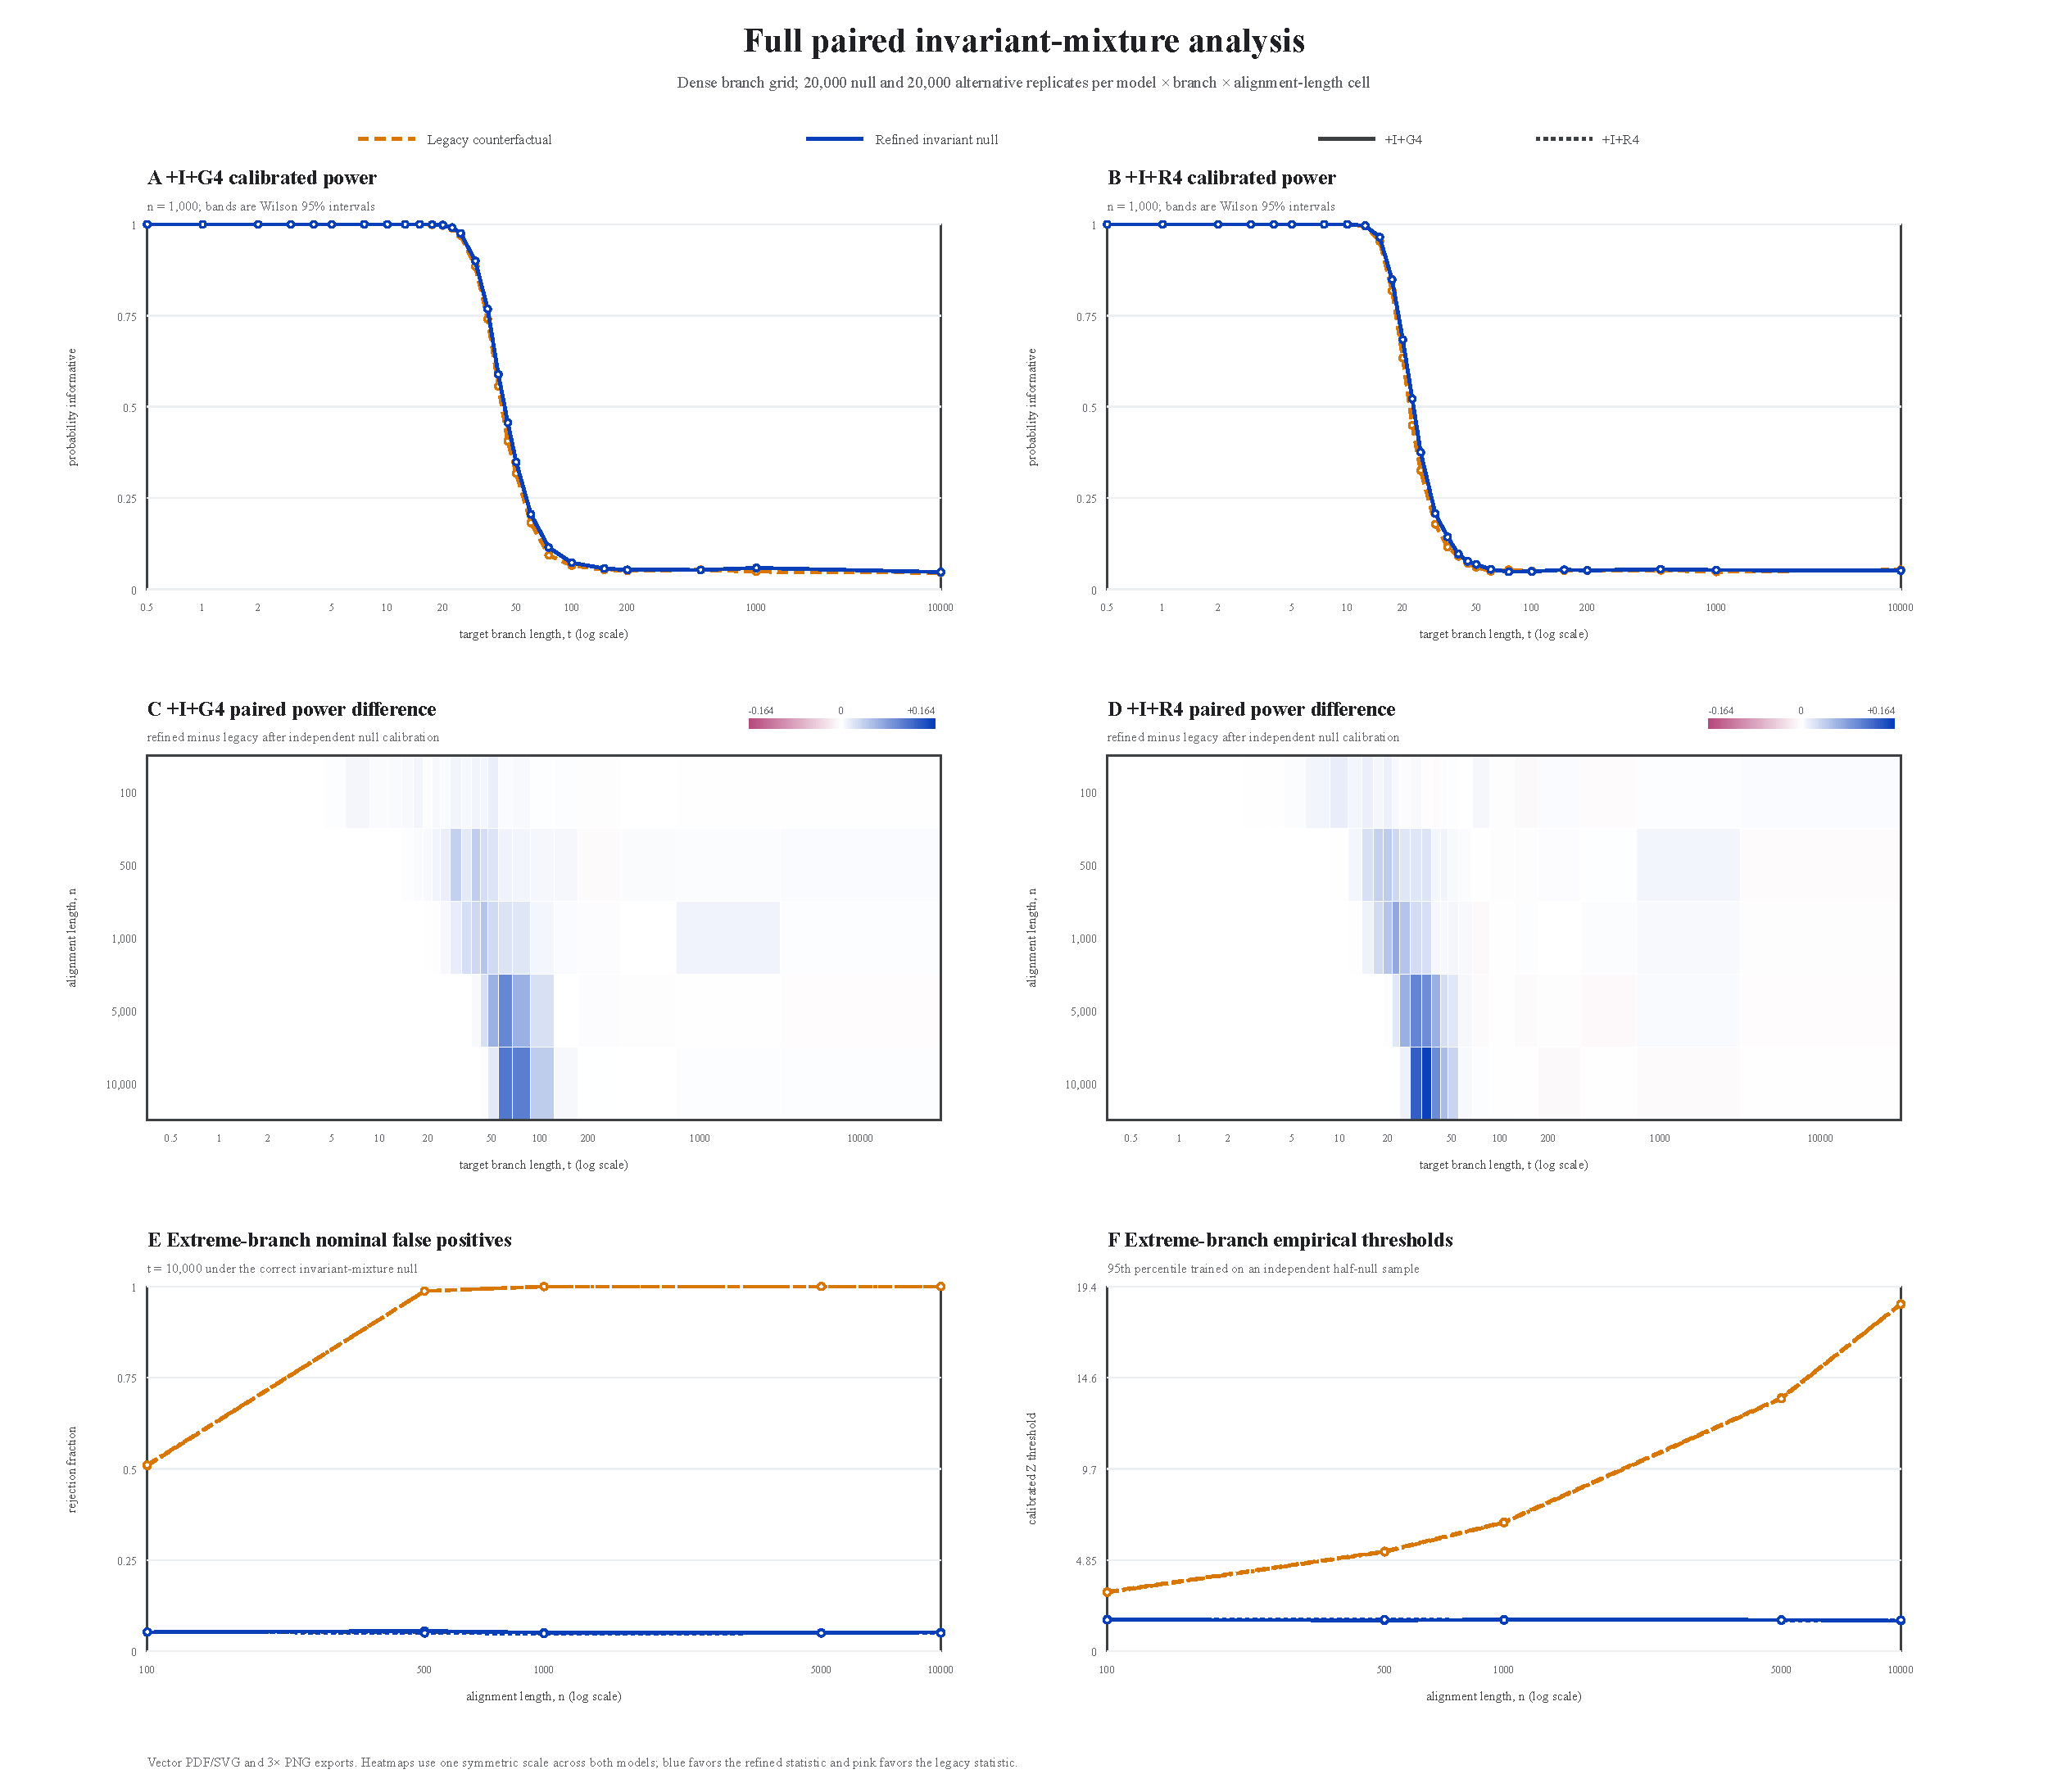
\includegraphics[width=1.08\textwidth]{figures/figure_weighted_invariant_full.pdf}}
  \caption{\textbf{Full paired \(+I+G4\) and \(+I+R4\) invariant-mixture analysis.} \textbf{a,b,} Formula-specific empirically calibrated power at 1,000 sites across the 27-step branch grid; bands are Wilson 95\% intervals. \textbf{c,d,} Refined-minus-counterfactual calibrated power for all five alignment lengths. Blue cells favor the refined statistic and pink cells favor the counterfactual statistic; both panels share one symmetric color scale. \textbf{e,} Nominal false-positive rates at \(t=10{,}000\). \textbf{f,} Formula-specific empirical 95th-percentile thresholds trained on an independent half-null sample.}
\end{figure}
